\documentclass[11pt]{article}
\usepackage{graphicx}
\usepackage{hyperref}
\usepackage{natbib}

\setlength{\textwidth}{6.5in}
\setlength{\headheight}{0in}
\setlength{\textheight}{8.0in}
\setlength{\hoffset}{0in}
\setlength{\voffset}{0in}
\setlength{\oddsidemargin}{0in}
\setlength{\evensidemargin}{0in}

\title{PS2}
  
\author{Shihong Pan}


\begin{document}

\maketitle

\section{Q1}
Fig \ref{fig:Q1} is the output for Q1. 

\section{Q2}
Fig \ref{fig:Q2} is the output for Q2. I found those exponents just by trial and error.


\section{Q3}
See the output of the two versions in Fig \ref{fig:Q3}. The no-for-loop version runs faster. The value of $L$ used is 100.
  
\section{Q4}
The Mandelbrot set is plotted in Fig \ref{fig:Q4}. I used 100 iterations for each c and $N=2000$. The running time was between 30 and 60 seconds which is within the acceptable range as described in the exercise.

\section{Q5}
\subsection{part a}
Fig \ref{fig:Q5ab} shows the solutions of the given quadratic equation. It also contains the solutions for part b.
\subsection{part b}
\begin{equation}
    x = \frac{-b\pm\sqrt{b^2-4ac}}{2a}\times\frac{-b\mp\sqrt{b^2-4ac}}{-b\mp\sqrt{b^2-4ac}} = \frac{b^2-(b^2-4ac)}{-2ab\mp2a\sqrt{b^2-4ac}}=\frac{2c}{-b\mp\sqrt{b^2-4ac}}
\end{equation}
The solutions obtained using the new form of $x$ are shown in Fig \ref{fig:Q5ab}. I see that there are discrepancies between the solutions and their order of magnitude are quite different (the difference between the first ones is on the order of 1e-7, while that between the second ones is on the order of 1e1). This happens because the value of $b$ is relatively large compared to the values of $a$ and $c$, such that $\sqrt{b^2-4ac}\approx b$. Thus in part a, the first solution has small number divided by small number, the second solution has large (in terms of magnitude) number divided by small number. In part b, the first solution has small number divided by large number, the second solution has small number divided by small number.

\subsection{part c}
My quadratic module passed the test. The output is in Fig \ref{fig:Q5c}


\begin{figure}[b!]
\centering
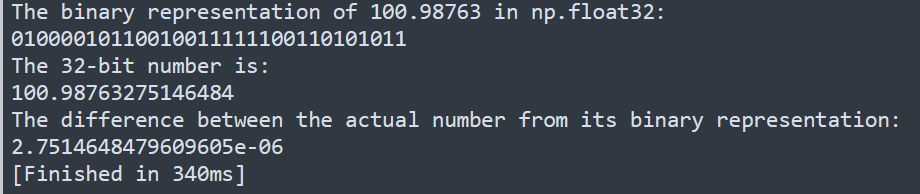
\includegraphics[width=0.7\textwidth]{Computational Physics/q1Output.PNG}
\caption{Q1 answer}
  \label{fig:Q1}
\end{figure}

\begin{figure}[b!]
\centering
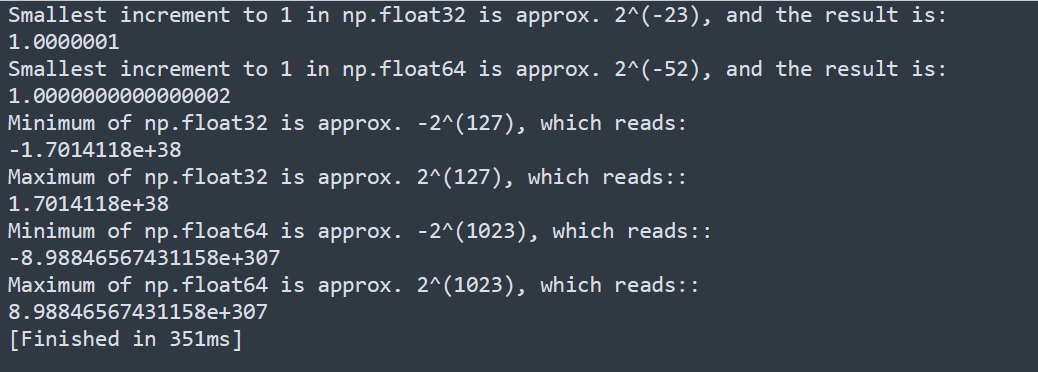
\includegraphics[width=0.7\textwidth]{Computational Physics/q2Output.PNG}
\caption{Q2 answer}
  \label{fig:Q2}
\end{figure}

\begin{figure}[b!]
\centering
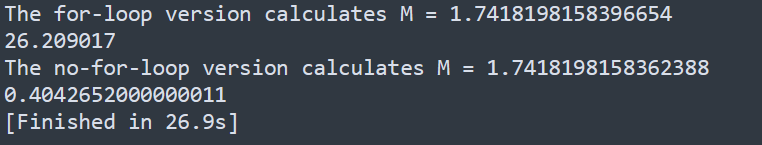
\includegraphics[width=0.7\textwidth]{Computational Physics/q3Output.PNG}
\caption{The value of M is the value of the Madelung constant of NaCl. The two numbers 26.209017 and 0.404265 are the running time of the for-loop version and the no-for-loop version respectively.}
  \label{fig:Q3}
\end{figure}

\begin{figure}[b!]
\centering
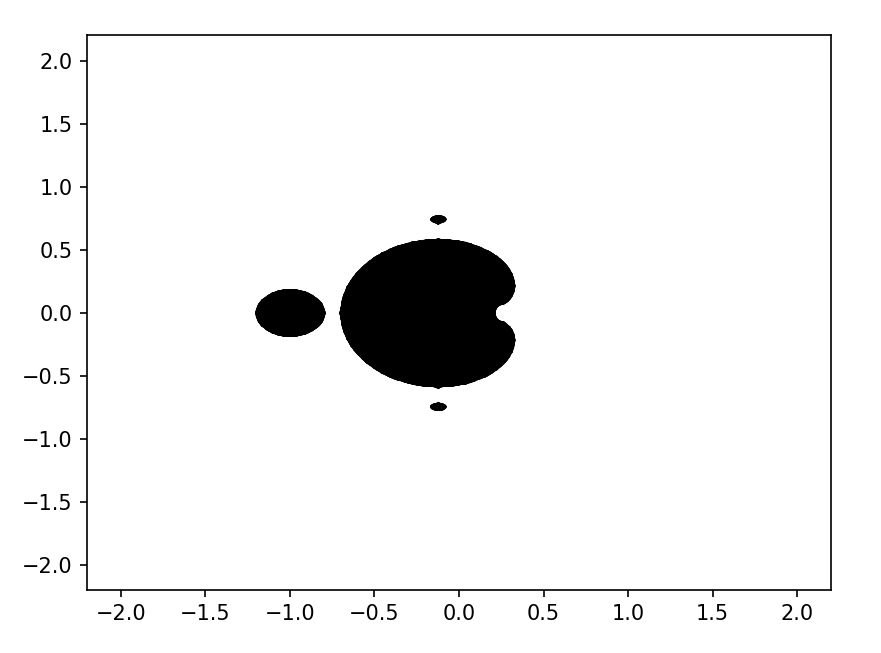
\includegraphics[width=0.7\textwidth]{Computational Physics/q4Output.PNG}
\caption{The plot for Q4.}
  \label{fig:Q4}
\end{figure}

\begin{figure}[b!]
\centering
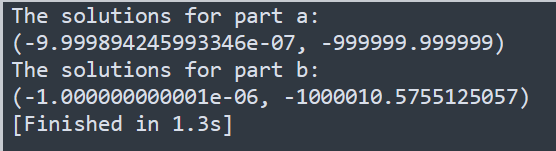
\includegraphics[width=0.7\textwidth]{Computational Physics/q5abOutput.PNG}
\caption{The solutions of the given quadratic equation, for both part a and part b.}
  \label{fig:Q5ab}
\end{figure}

\begin{figure}[b!]
\centering
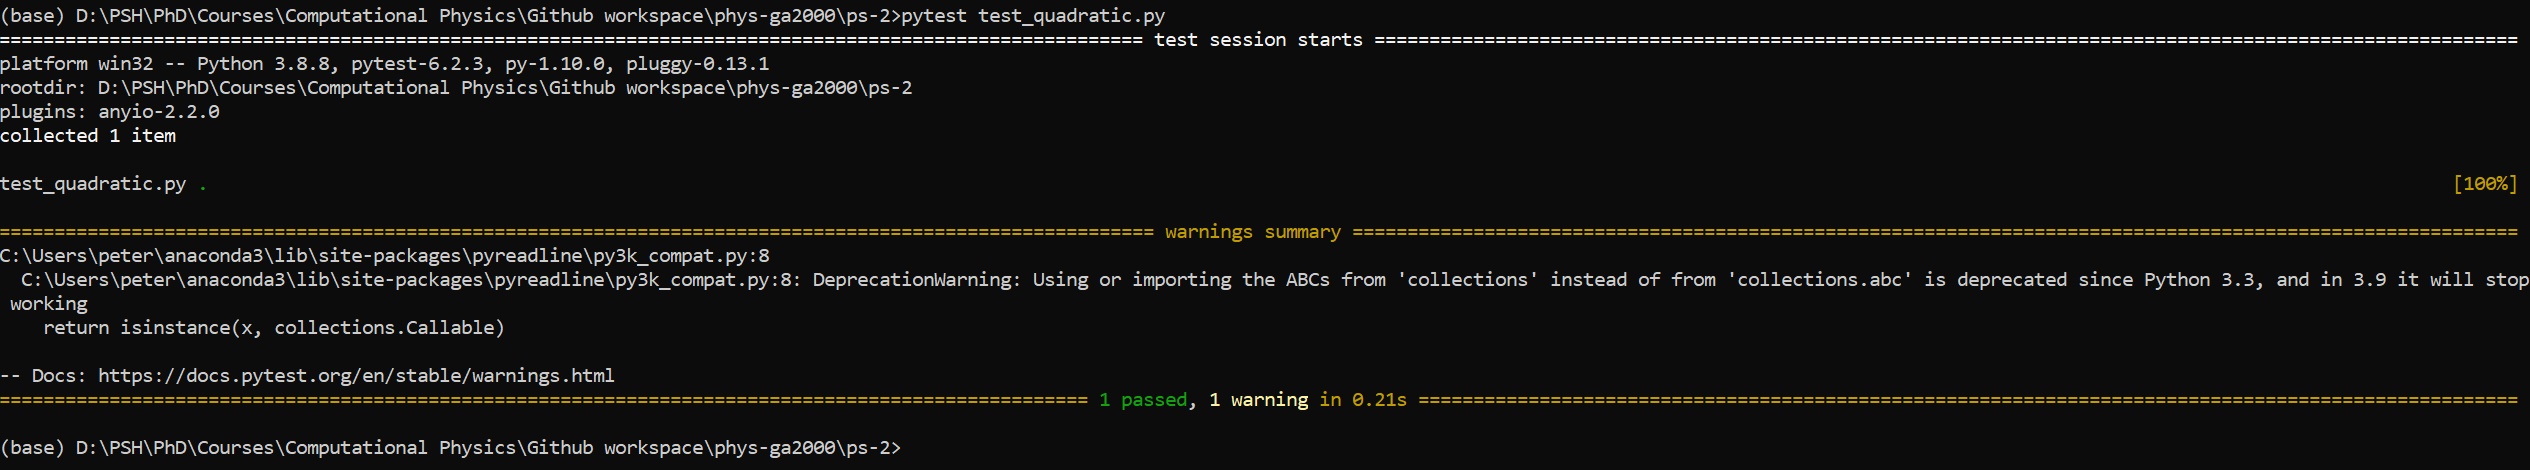
\includegraphics[width=0.9\textwidth]{Computational Physics/q5cOutput.PNG}
\caption{The output of pytest test\_quadratic.py.}
  \label{fig:Q5c}
\end{figure}



\bibliographystyle{apj}
\bibliography{example}

\end{document}

 
 
